\begin{frame}{Árvore binária de busca}
    \metroset{block=fill}

    Existem algumas técnicas para, após uma inserção ou remoção, rebalancear a árvore com complexidade $O(\log n)$. Veja o capítulo $13$ do Cormen.

    Para uma mesma lista $l$, é possível criar várias árvores binárias de busca possuindo nós com os valores de $l$. Por exemplo, se $l = \{1, 2, 3, 4\}$, então temos

    \begin{columns}
        \begin{column}{0.25\textwidth}
            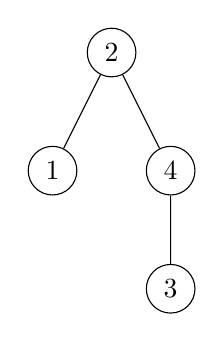
\begin{tikzpicture}[every node/.style={circle, draw=black}]
                \node {2}
                    child { node {1} }
                    child { node {4} 
                        child {node {3}}
                    }
                ;
            \end{tikzpicture}
        \end{column}
        \begin{column}{0.25\textwidth}
            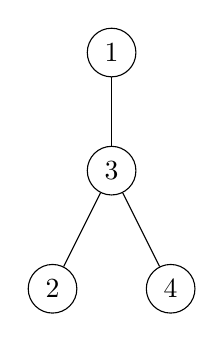
\begin{tikzpicture}[every node/.style={circle, draw=black}]
                \node {1}
                    child { node {3} 
                        child {node {2}}
                        child {node {4}}
                    }
                ;
            \end{tikzpicture}
        \end{column}
    \end{columns}


\end{frame}